% ══════════════════════════════════════════════════════
% PHẦN 1 — MỞ ĐẦU, NỀN TẢNG, KIẾN TRÚC
% Người thuyết trình: A (TV2 — Đoàn Hồng Bảo)
% Phong cách: Tối giản (Minimum) — Keyword + Biểu tượng
% ══════════════════════════════════════════════════════

\section{Mở đầu \& Nền tảng}

% ── Slide 1: Bài toán thực tế ──────────────────────────
\begin{frame}{Bài toán thực tế: Dữ liệu dạng đồ thị}
  \vspace{0.2em}
  \begin{columns}[c]
    \begin{column}{0.50\textwidth}
      \centering
      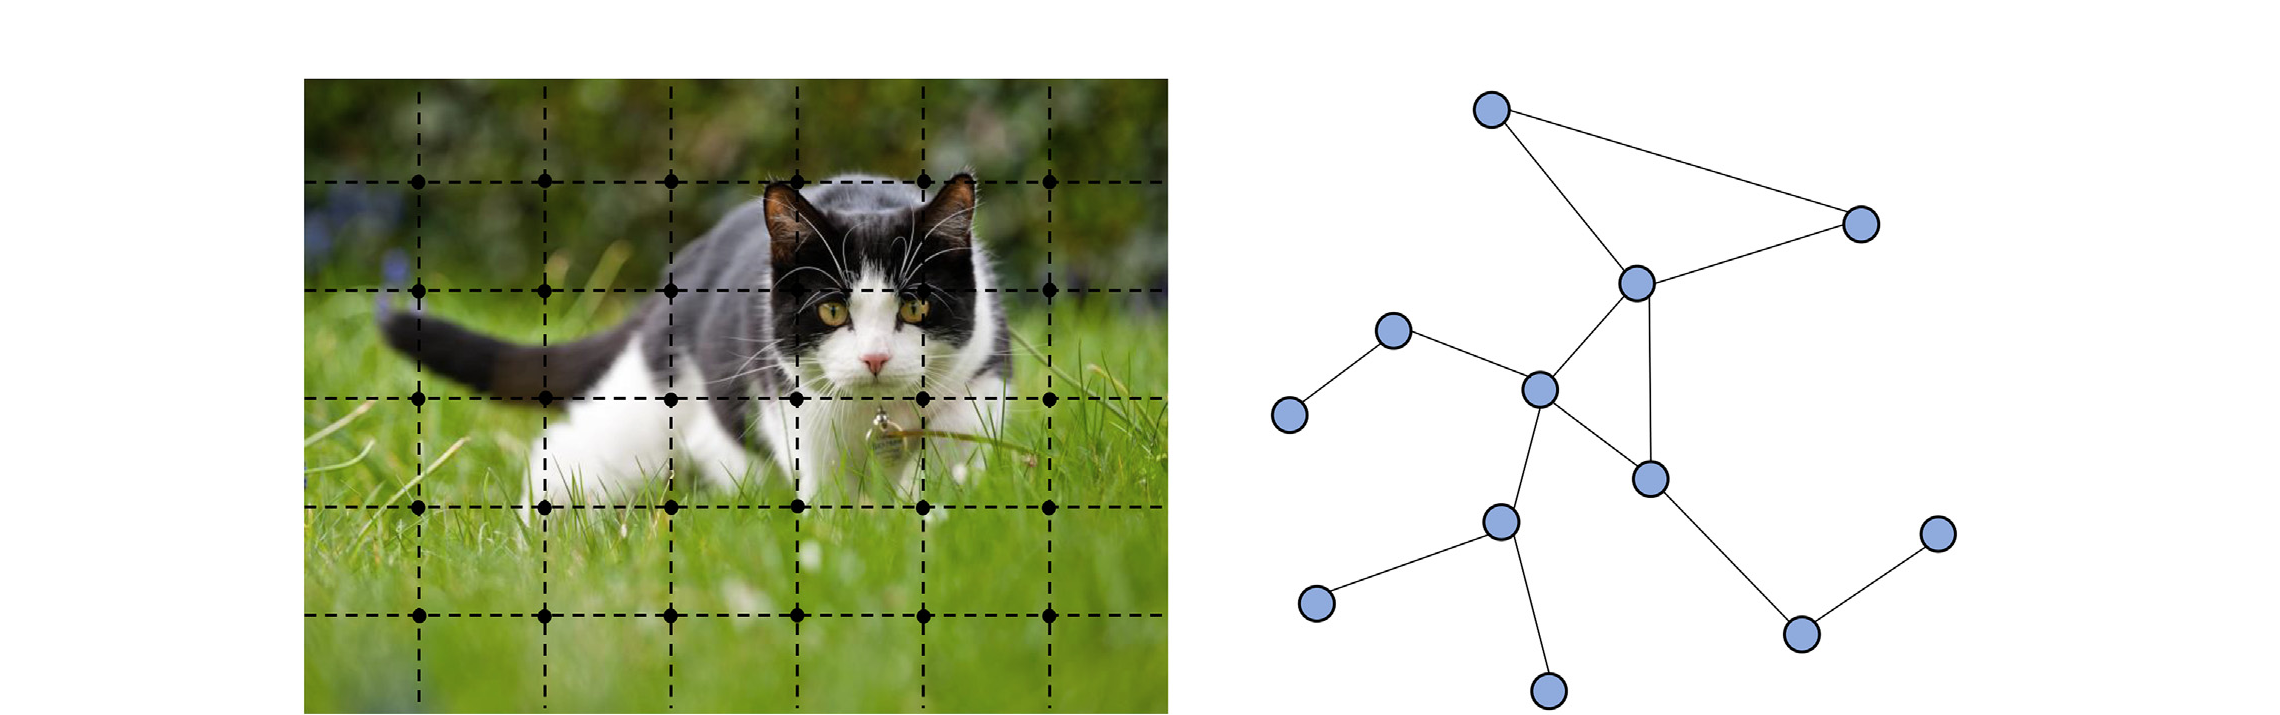
\includegraphics[width=\linewidth, height=0.36\textheight, keepaspectratio]{gnn/fig1_graph.png}
      \vspace{0.3em}

      {\footnotesize\textit{Zhou et al. (2020), Fig. 1: Ảnh (Euclidean) vs.\ Đồ thị (non-Euclidean)}}
    \end{column}

    \begin{column}{0.48\textwidth}
      \textcolor{Theme_Color}{\textbf{\large Ví dụ \& Bài toán}}
      \vspace{0.5em}
      \begin{itemize}
        \setlength{\itemsep}{0.5em}
        \item \textbf{Ví dụ:} Mạng xã hội $\cdot$ Mạng trích dẫn $\cdot$ Phân tử $\cdot$ Giao thông
        \item \textbf{Bài toán:} Phân loại nút — dự đoán nhãn từng nút
        \item \textbf{Thách thức:} Nhãn \textbf{đắt đỏ}, đồ thị \textbf{lớn} $\rightarrow$ thiếu dữ liệu giám sát
        \item \textcolor{orange!85!black}{\textbf{Hệ quả:}} Học biểu diễn \textbf{không giám sát} $\rightarrow$ \textbf{SSL}
      \end{itemize}
    \end{column}
  \end{columns}
\end{frame}


% ── Slide 2: Bài toán Đồ thị & SSL ─────────────────────
\begin{frame}{Bài toán Đồ thị \& Học tự giám sát (SSL)}
  \vspace{0.2em}
  \begin{columns}[c]
    \begin{column}{0.46\textwidth}
      \centering
      \begin{tikzpicture}[
        scale=0.88,
        nd/.style={circle, fill=Theme_Color!75, draw=Theme_Color, text=white, inner sep=0pt, minimum size=18pt, font=\scriptsize\bfseries},
        nd2/.style={circle, fill=orange!80, draw=orange!90!black, text=white, inner sep=0pt, minimum size=18pt, font=\scriptsize\bfseries},
        ed/.style={thick, gray!65}
      ]
        \node[nd] (v1) at (0, 1.1) {$v_1$};
        \node[nd] (v2) at (-1.3, 0.2) {$v_2$};
        \node[nd2] (v3) at (1.3, 0.2) {$v_3$};
        \node[nd2] (v4) at (-0.8, -1.0) {$v_4$};
        \node[nd] (v5) at (0.9, -1.0) {$v_5$};
        \draw[ed] (v1) -- (v2) (v1) -- (v3) (v2) -- (v4) (v3) -- (v5) (v2) -- (v5) (v4) -- (v5);
        \node[anchor=north, font=\scriptsize, text=black!75] at (0, -1.5) {$G=(V,E)$, \quad $X \in \mathbb{R}^{|V|\times d}$};
      \end{tikzpicture}
    \end{column}

    \begin{column}{0.52\textwidth}
      \textcolor{Theme_Color}{\textbf{\large Mô tả bài toán}}
      \vspace{0.5em}
      \begin{itemize}
        \setlength{\itemsep}{0.55em}
        \item \textbf{Đầu vào:} Đồ thị $G=(V,E)$ kèm đặc trưng nút $X$
        \item \textbf{Mục tiêu:} Học biểu diễn $X \xrightarrow{\text{học}} H \in \mathbb{R}^{|V|\times d'}$
        \item \textbf{Ứng dụng:} Phân loại nút $\cdot$ Phân cụm nút
      \end{itemize}
    \end{column}
  \end{columns}
\end{frame}


% ── Slide 3: GNN làm gì ───────────────────────────────
\begin{frame}{GNN: Từ láng giềng đến node embedding}
  \centering
  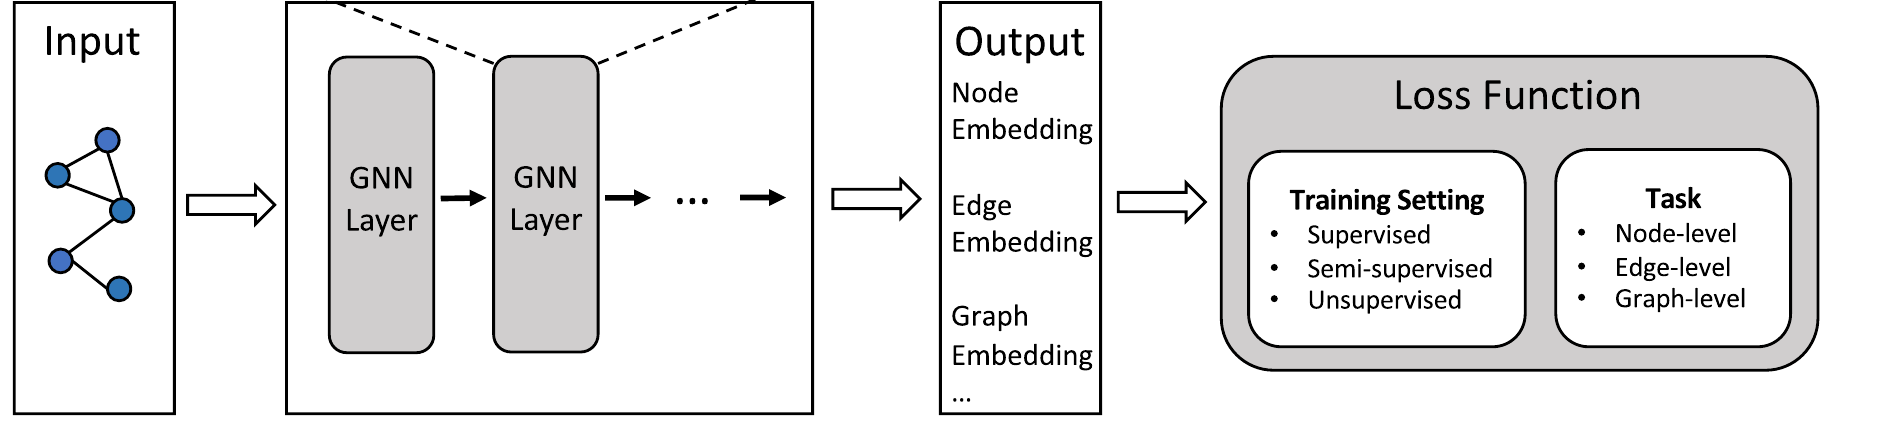
\includegraphics[width=\linewidth, keepaspectratio]{gnn/fig2_pipeline-v2.png}
  \vspace{0.3em}

  {\footnotesize\textit{Zhou et al. (2020), Fig. 2: pipeline tổng quát của GNN}}
\end{frame}


% ── Slide 4: Bức tranh Graph SSL ───────────────────────
\begin{frame}{Bức tranh Graph SSL: Contrastive vs.\ Generative}
  \vspace{0.3em}
  \centering
  \renewcommand{\arraystretch}{1.35}
  \small
  \begin{tabular}{p{2.1cm}p{5.2cm}p{5.2cm}}
    \toprule
    \textbf{Tiêu chí} & \textcolor{Theme_Color}{\textbf{Contrastive}} & \textcolor{orange!85!black}{\textbf{Generative}} \\
    \midrule
    \textbf{Ý tưởng} & Tạo 2 góc nhìn nhiễu, kéo cặp dương / đẩy cặp âm & Mã hóa đồ thị và tái tạo lại cấu trúc / đặc trưng \\
    \textbf{Đại diện} & DGI, GRACE, BGRL & GAE, MaskGAE, \textbf{GraphMAE} \\
    \textbf{Ưu điểm} & Học biểu diễn phân biệt tốt & Đơn giản, không cần augmentation phức tạp hay negative sampling \\
    \textbf{Nhược điểm} & Phụ thuộc phép tăng cường, tốn chi phí mẫu âm & Phụ thuộc mạnh vào ngữ cảnh láng giềng để tái tạo \\
    \bottomrule
  \end{tabular}
\end{frame}


% ── Slide 5: Graph Masked Autoencoder (GraphMAE) ──────
\begin{frame}{Generative methods}
  \centering
  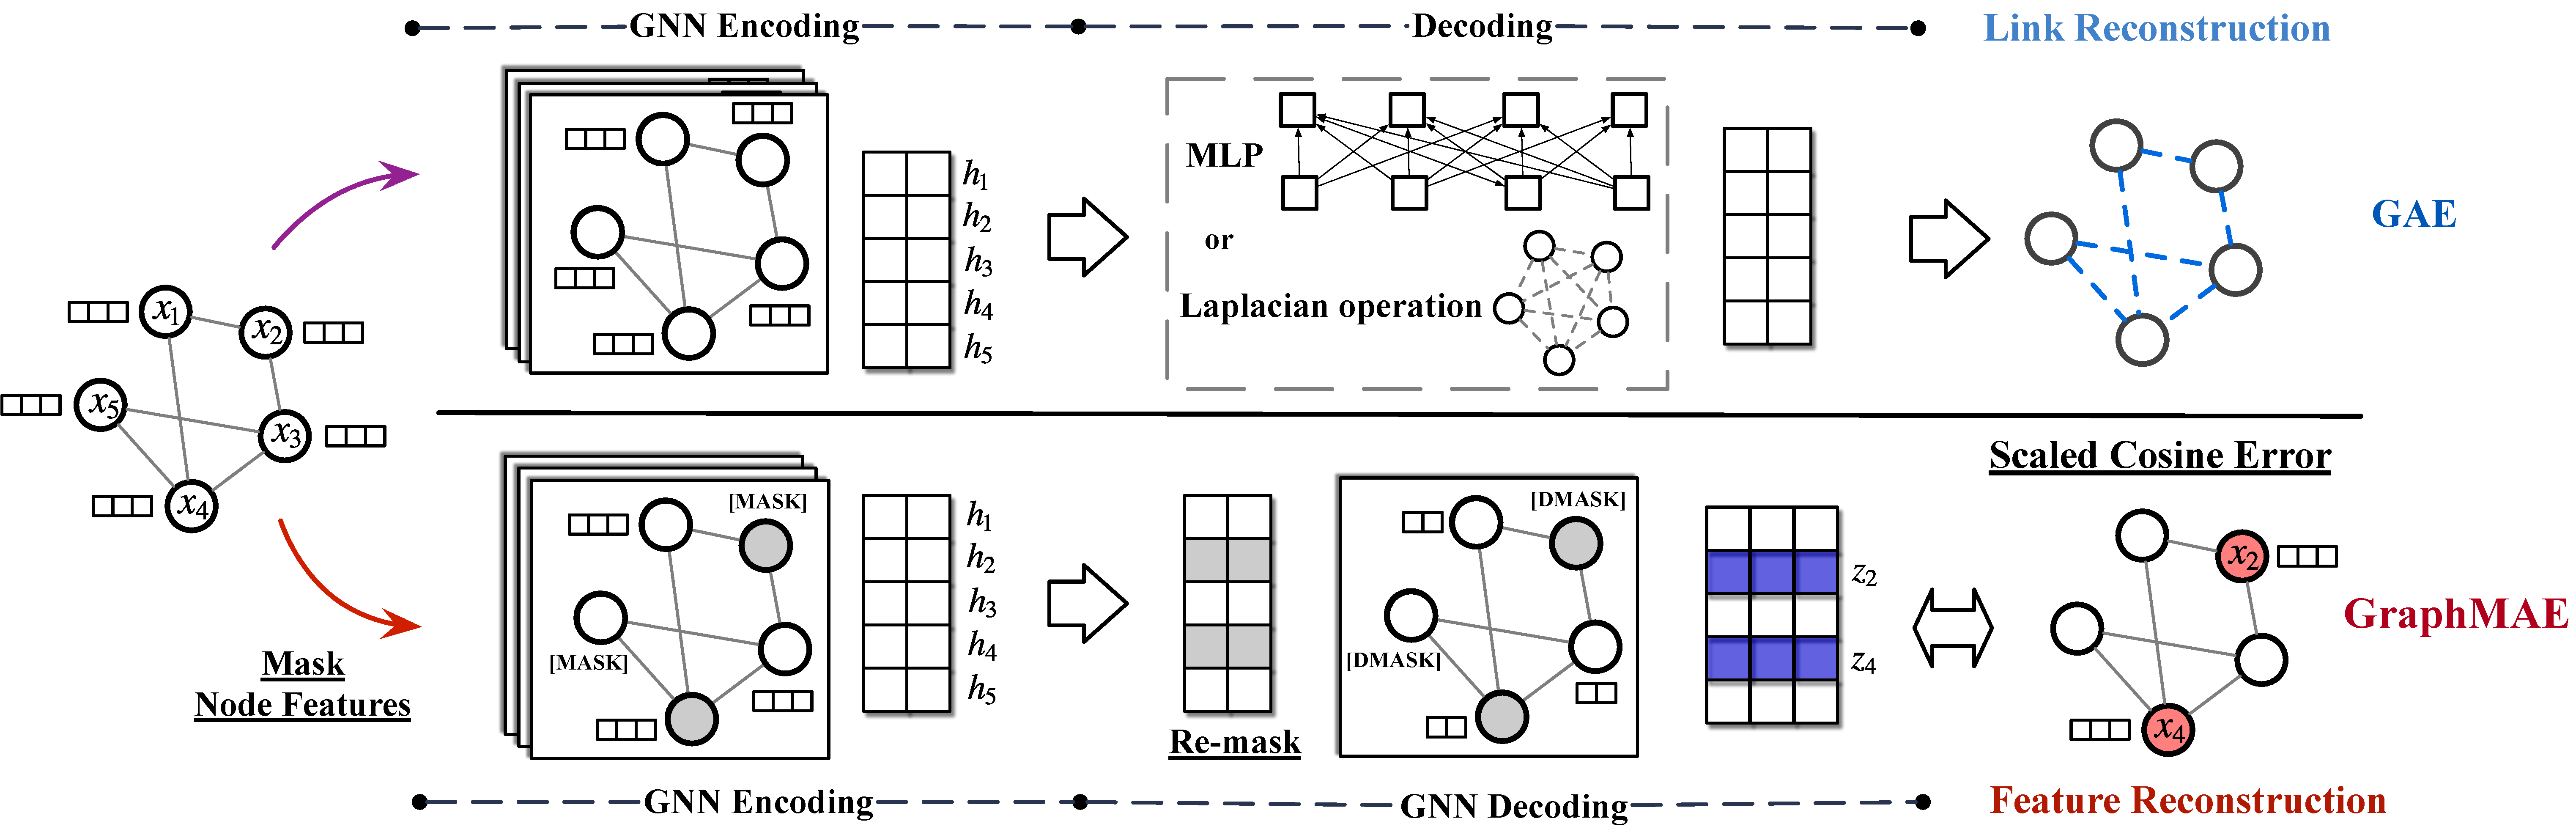
\includegraphics[width=0.84\linewidth, height=0.38\textheight, keepaspectratio]{arXiv-2205.10803v3/imgs/overview.pdf}
  \vspace{0.3em}

  \begin{columns}[T]
    \begin{column}{0.46\textwidth}
      \textcolor{Theme_Color}{\textbf{\small GAE — nhánh trên}}
      \vspace{0.3em}
      \begin{itemize}
        \setlength{\itemsep}{0.35em}
        \item Tái tạo \textbf{cạnh}: $A \rightarrow \hat{A}$
        \item Encoder GNN $\rightarrow$ decoder MLP
      \end{itemize}
    \end{column}

    \begin{column}{0.48\textwidth}
      \textcolor{orange!85!black}{\textbf{\small GraphMAE — nhánh dưới}}
      \vspace{0.3em}
      \begin{itemize}
        \setlength{\itemsep}{0.35em}
        \item Che đặc trưng nút: $X \rightarrow \hat{X}$
        \item Tái tạo \textbf{đặc trưng}, loss \textbf{SCE}
      \end{itemize}
    \end{column}
  \end{columns}
\end{frame}


% ── Slide 6: Đồng tính vs Dị tính — Định nghĩa ────────
\begin{frame}{Tính đồng tính vs.\ Tính dị tính: Định nghĩa}
  \vspace{0.2em}
  \begin{columns}[T]
    \begin{column}{0.48\textwidth}
      \textcolor{Theme_Color}{\textbf{\large Homophily (Đồng tính)}}
      \vspace{0.4em}
      \begin{itemize}
        \setlength{\itemsep}{0.4em}
        \item Phần lớn cạnh nối nút \textbf{cùng nhãn} ($y_i = y_j$)
        \item Tỉ lệ đồng tính $h$ \textbf{cao}
      \end{itemize}
      \vspace{0.5em}
      \centering
      \begin{tikzpicture}[
        scale=0.85,
        na/.style={circle, fill=Theme_Color!75, draw=Theme_Color, text=white, inner sep=0pt, minimum size=15pt, font=\scriptsize\bfseries},
        nb/.style={circle, fill=orange!80, draw=orange!90!black, text=white, inner sep=0pt, minimum size=15pt, font=\scriptsize\bfseries},
        ehomo/.style={thick, Theme_Color!80},
        ehet/.style={thick, orange!85!black, dashed}
      ]
        \node[na] (a1) at (0, 0.9) {$A$};
        \node[na] (a2) at (-1.1, 0) {$A$};
        \node[na] (a3) at (1.1, 0) {$A$};
        \node[na] (a4) at (0, -0.8) {$A$};
        \node[nb] (b1) at (2.2, 0.5) {$B$};
        \draw[ehomo] (a1) -- (a2);
        \draw[ehomo] (a1) -- (a3);
        \draw[ehomo] (a2) -- (a4);
        \draw[ehomo] (a3) -- (a4);
        \draw[ehomo] (a1) -- (a4);
        \draw[ehet]  (a3) -- (b1);
        \node[anchor=north, font=\scriptsize, text=black!70] at (0.5, -1.45) {$h = 5/6$};
      \end{tikzpicture}
    \end{column}

    \begin{column}{0.48\textwidth}
      \textcolor{orange!85!black}{\textbf{\large Heterophily (Dị tính)}}
      \vspace{0.4em}
      \begin{itemize}
        \setlength{\itemsep}{0.4em}
        \item Phần lớn cạnh nối nút \textbf{khác nhãn} ($y_i \neq y_j$)
        \item Tỉ lệ đồng tính $h$ \textbf{thấp}
      \end{itemize}
      \vspace{0.5em}
      \centering
      \begin{tikzpicture}[
        scale=0.85,
        na/.style={circle, fill=Theme_Color!75, draw=Theme_Color, text=white, inner sep=0pt, minimum size=15pt, font=\scriptsize\bfseries},
        nb/.style={circle, fill=orange!80, draw=orange!90!black, text=white, inner sep=0pt, minimum size=15pt, font=\scriptsize\bfseries},
        ehomo/.style={thick, Theme_Color!80},
        ehet/.style={thick, orange!85!black, dashed}
      ]
        \node[na] (a1) at (0, 0.9) {$A$};
        \node[nb] (b1) at (-1.1, 0) {$B$};
        \node[nb] (b2) at (1.1, 0) {$B$};
        \node[na] (a2) at (0, -0.8) {$A$};
        \node[na] (a3) at (2.2, 0.5) {$A$};
        \draw[ehet]  (a1) -- (b1);
        \draw[ehet]  (a1) -- (b2);
        \draw[ehet]  (b1) -- (a2);
        \draw[ehet]  (b2) -- (a2);
        \draw[ehet]  (b2) -- (a3);
        \draw[ehomo] (b1) -- (b2);
        \node[anchor=north, font=\scriptsize, text=black!70] at (0.5, -1.45) {$h = 1/6$};
      \end{tikzpicture}
    \end{column}
  \end{columns}

  \vspace{0.4em}
  \centering
  {\footnotesize Nét liền: cùng nhãn $\cdot$ Nét đứt: khác nhãn}\\[0.3em]
  $h = \dfrac{|\{(i,j) \in E : y_i = y_j\}|}{|E|}$
\end{frame}


% ── Slide 7: Vấn đề của GMAE trên đồ thị dị tính ─────
\begin{frame}{Vấn đề: Điểm yếu của GMAE trên đồ thị dị tính}
  \begin{columns}[T]
    \begin{column}{0.46\textwidth}
      \centering
      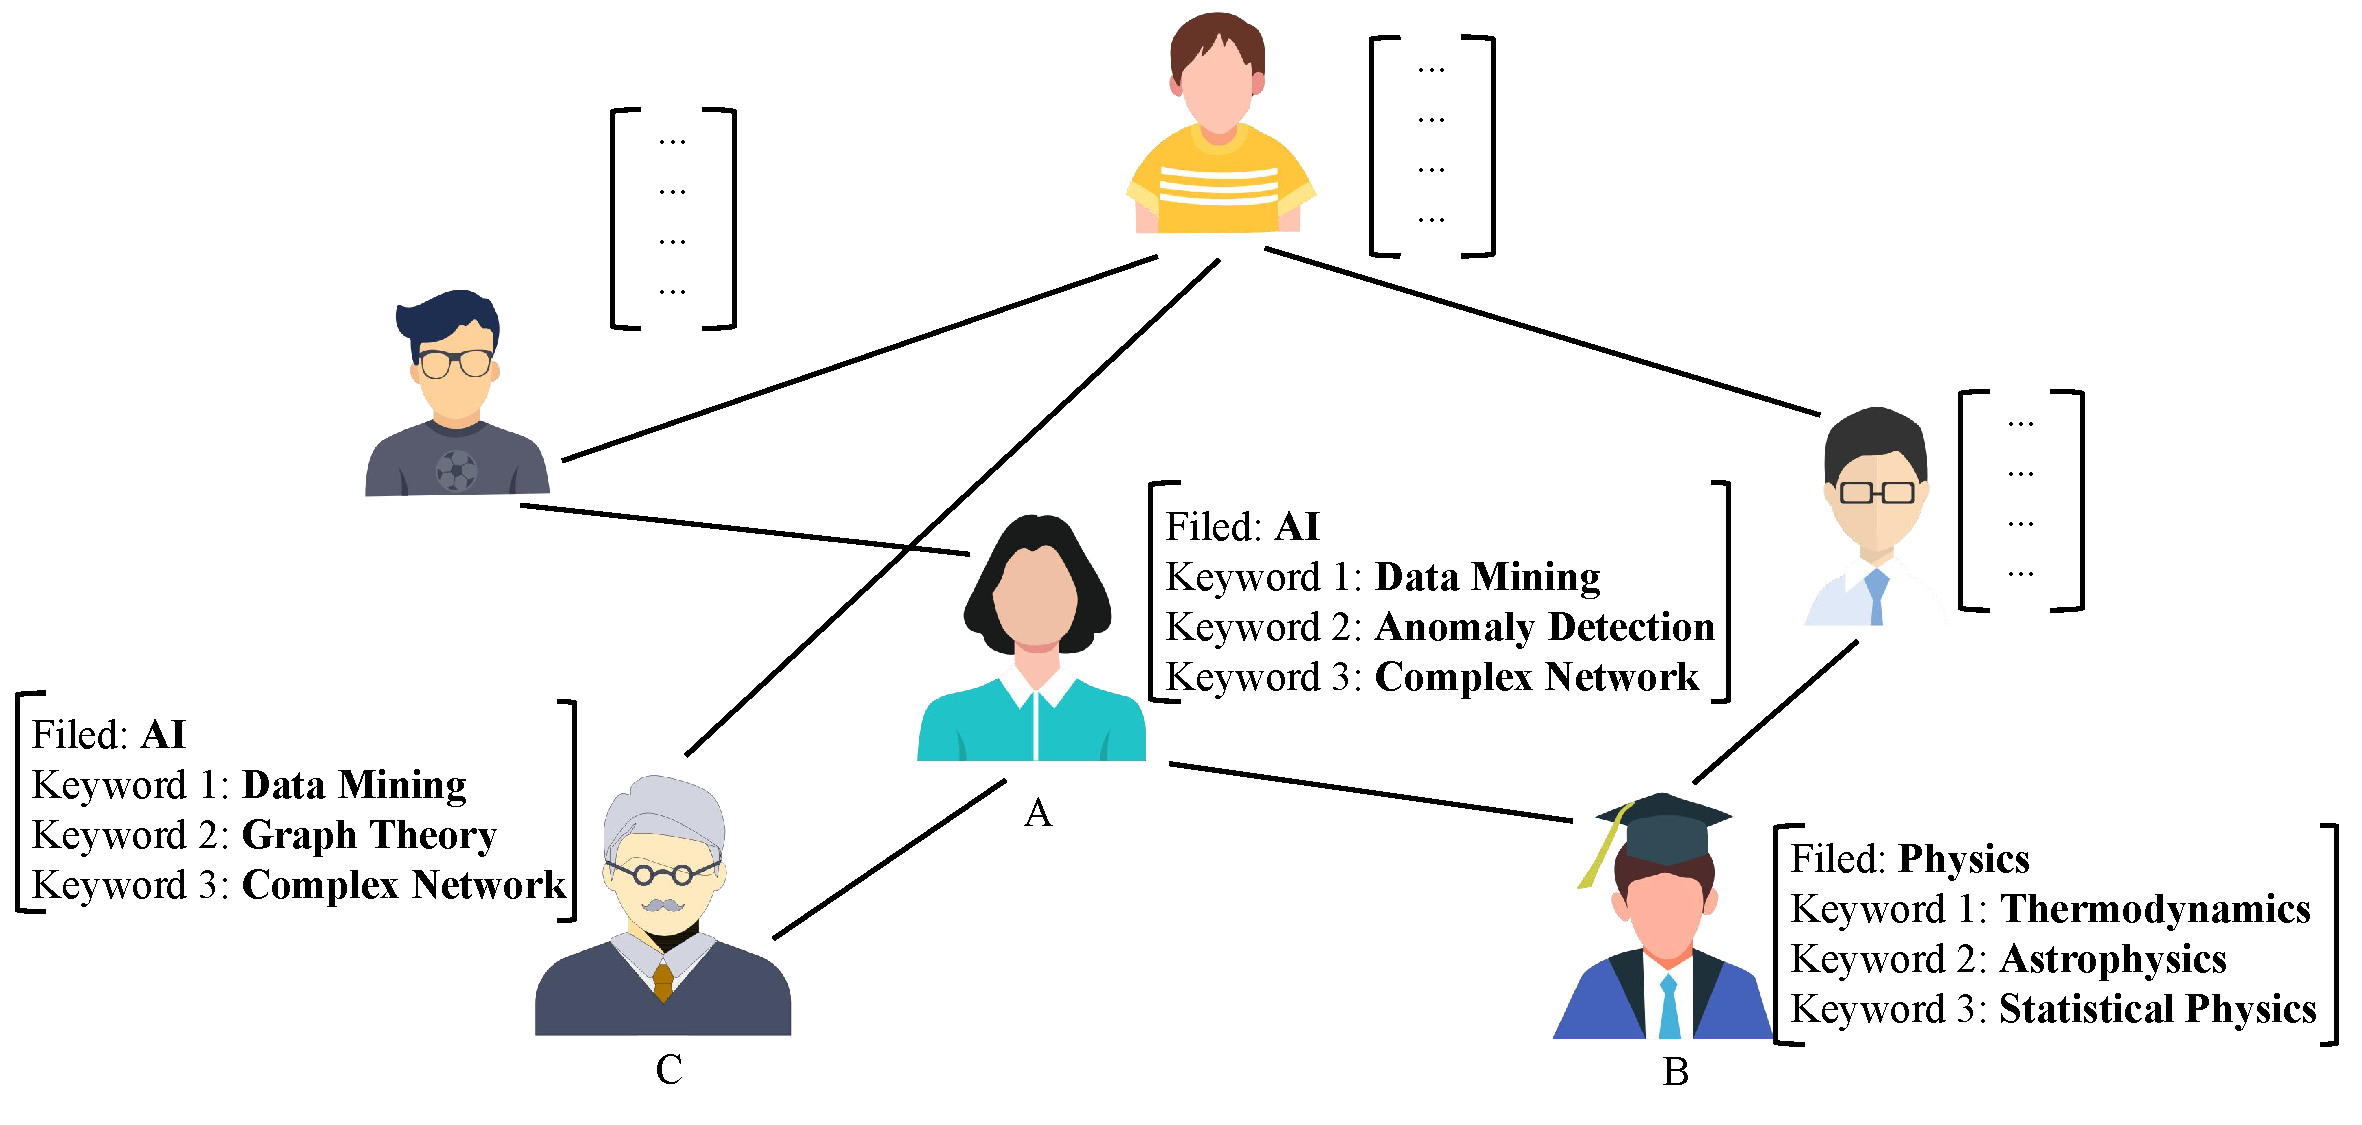
\includegraphics[width=\linewidth, height=0.45\textheight, keepaspectratio]{example.pdf}
      \vspace{0.4em} \\
      \small
      A (AI) $\leftrightarrow$ C (AI), B (Vật lý) \\
      Che A $\rightarrow$ B gây \textcolor{orange!85!black}{\textbf{nhiễu}}
    \end{column}

    \begin{column}{0.50\textwidth}
      \textcolor{orange!85!black}{\textbf{\large Điểm yếu cốt lõi}}
      \vspace{0.5em}
      \begin{itemize}
        \setlength{\itemsep}{0.6em}
        \item Thiên về \textbf{nhất quán (Consistency)}
        \item Thiếu \textbf{sai khác (Discrepancy)}
        \item Kéo nút khác lớp lại \textbf{gần nhau}
      \end{itemize}
    \end{column}
  \end{columns}
\end{frame}


% ── Slide 8: Thực nghiệm chứng minh vấn đề ────────────
\begin{frame}{Thực nghiệm chứng minh: Xóa nhòa sự khác biệt}
  \begin{columns}[T]
    \begin{column}{0.45\textwidth}
      \centering
      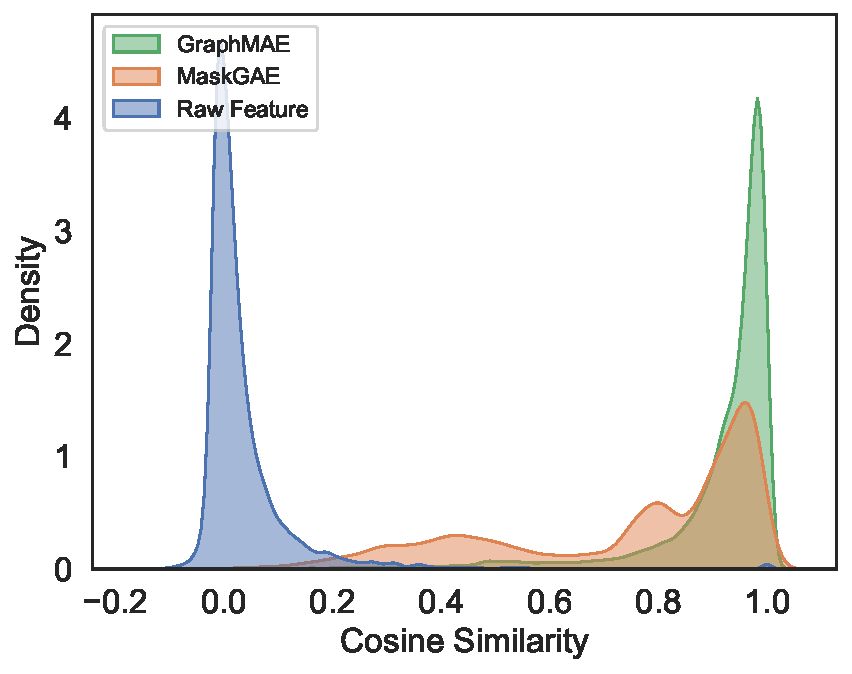
\includegraphics[width=\linewidth, height=0.55\textheight, keepaspectratio]{fig1.pdf}
      \vspace{0.2em} \\
      {\footnotesize\textit{Figure 2: Cosine similarity trên Squirrel}}
    \end{column}

    \begin{column}{0.52\textwidth}
      \textcolor{Theme_Color}{\textbf{\large Quan sát (Cặp nút khác lớp)}}
      \vspace{0.5em}
      \begin{itemize}
        \setlength{\itemsep}{0.6em}
        \item \textbf{Raw features:} $\approx 0$
        \item \textbf{GraphMAE / MaskGAE:} $\longrightarrow 1$
      \end{itemize}

      \vspace{0.8em}
      \textcolor{orange!85!black}{\textbf{\large Kết luận}}
      \vspace{0.4em}
      \begin{itemize}
        \item Tăng độ tương đồng nút khác lớp
        \item Giảm khả năng phân biệt biểu diễn
      \end{itemize}
    \end{column}
  \end{columns}
\end{frame}


% ── Slide 9: Động lực phát triển DGMAE ────────────────
\begin{frame}{Động lực phát triển: Thách thức \& Đóng góp của DGMAE}
  \vspace{0.3em}
  \textcolor{Theme_Color}{\textbf{\large Đóng góp (DGMAE)}}
  \vspace{0.6em}
  \begin{itemize}
    \setlength{\itemsep}{0.7em}
    \item \textbf{Tư duy mới:} Consistency $\rightarrow$ \textbf{Preserve Discrepancy}
    \item \textbf{Adaptive Selection:} Dùng attention chọn cạnh sai khác
    \item \textbf{Hiệu năng:} Tốt nhất \textbf{16/17} bộ dữ liệu
  \end{itemize}
\end{frame}


\section{Kiến trúc DGMAE}

% ── Slide 10: Kiến trúc tổng thể DGMAE ────────────────
\begin{frame}{Kiến trúc tổng thể DGMAE (Figure 3)}
  \centering
  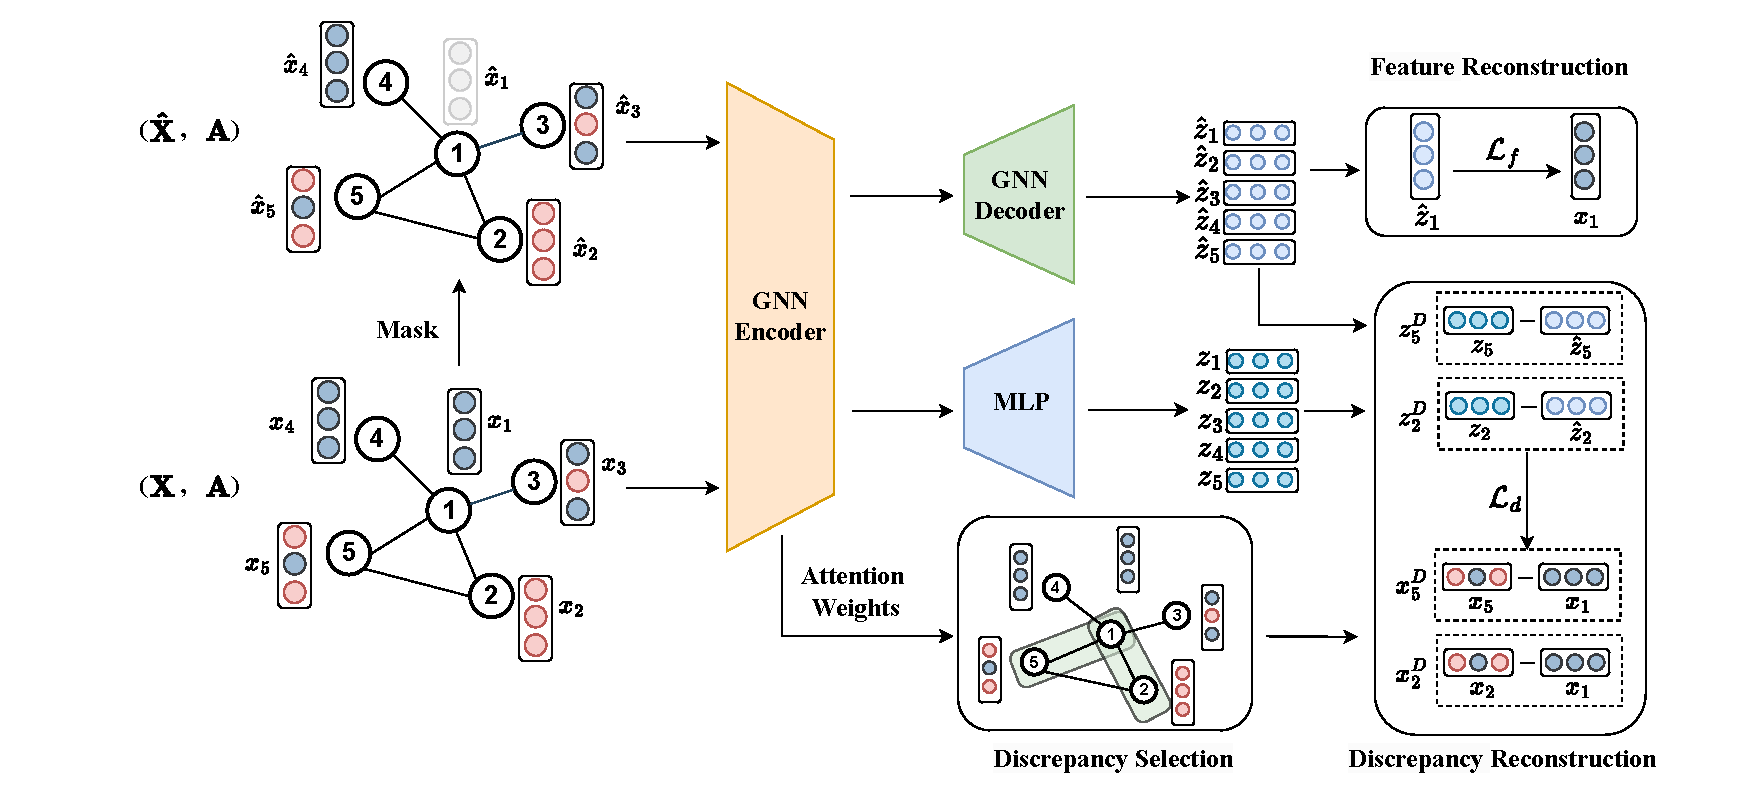
\includegraphics[width=0.92\linewidth, height=0.58\textheight, keepaspectratio]{model.pdf}
  \vspace{0.8em}

  {\large \textbf{2 Nhánh song song:} \quad Feature Recon. ($\mathcal{L}_f$) \quad $+$ \quad Discrepancy Recon. ($\mathcal{L}_d$)}

\end{frame}


